
% ♥♥♥♥	♥♥♥♥
Les VBOs\footnote{http://raptor.developpez.com/tutorial/opengl/vbo/} (Vertex Buffer Object) en OpenGL est une méthode qui permet d'envoyer des données vers la carte graphique, elle remplace les VA (Vertex Array) déclarés comme obsolètes par OpenGL qui étaient enregistrés sur le CPU et devaient transiter entre CPU et GPU.\\
Les VBOs ont été conçus afin d'optenir les meilleurs performances possibles. Son utilisation est actuellement la méthode la plus efficace en OpenGL car les données 3D ne résident plus dans la mémoire système mais dans la mémoire de la carte graphique ce qui permet un rendu plus rapide.\\
Les VAOs (Vertex Array Object) servent à optimiser l'utilisation des VBOs, ils sont une fonctionnalité toute nouvelle qui ressemble fortement aux Display Lists. Les VAOs permettent la "sauvegarde" de plusieurs commandes dans un seul et même objet qui lui même sera stocké dans la mémoire de la carte graphique. \\
Par exemple : ces commandes ou appels de fonctions peuvent utiliser des VBOs. Ainsi tout sera stocké directement dans la carte graphique et celle-ci n'aura plus à demander à l'application ce qu'elle doit faire. OpenGL pourra ainsi optimiser ses actions du faite qu'il connetra ses actions futurs. Ceci permet d'éviter de faire transiter trop d'informations entre le système et la carte graphique.\\\\
La création d’un VBO suit les étapes suivantes : 
\begin{itemize}
\item La génération du nouveau buffer object avec \verb|glGenBuffersARB ( );|
\item L’activation du buffer object avec \verb|glBindBufferARB ( );|
\item La copie de la donnée du vertex au buffer object avec \verb|glBufferDataARB ( );| 
\item L’usage du buffer pour le rendu de la donnée
\item La destruction du buffer
\end{itemize}
\subsubsection*{La fonction glGenBuffers} 
Créé le buffer object et retourne un nombre d’identifiants du buffer object. Deux paramètres sont attendus : 
\verb|void glGenBuffers(GLsizei n, GLuint *buffers);|
\\
Le premier, \verb|GLsizei n| où n renvoie au nombre de buffer object que l’on veut générer, et le second \verb|GLuint *buffers| qui renvoie les nombres identifiants de buffers dans un bloc mémoire commençant par buffers (élément simple ou tableau)

\subsubsection*{La fonction glBindBufferARB}

Une fois que le nom du buffer object est généré, il faut l’activer pour ensuite l’utiliser. La fonction utile est 
\begin{center}
\verb|void glBindBuffer(GLenum type, Gluint buffer) ;|
\end{center}
qui prend en compte deux paramètres. \verb|GLenum type| où type peut être \verb|GL_ARRAY_BUFFER| ou \verb|GL_ELEMENT_ARRAY_BUFFER| (d’autres types sont connus, comme \verb|GL_PIXEL_PACK_BUFFER| mais leur utilisation se fait avec le Pixel Buffer Object (PBO) que nous n’aborderons pas ici). \verb|GL_ARRAY_BUFFER| est utilisé quand le buffer object se réfère aux données des vertex (positions, couleurs, normales etc.) \verb|GL_ELEMENT_ARRAY_BUFFER| est utilisé quand les indices des vertex seront stockés dans le buffer

\subsubsection*{La fonction glBufferData}

A présent le buffer object est généré et prêt à recevoir des données. Sa taille est par défaut mise à zéro, la fonction \verb|glBufferDate| sert donc à l’initialiser avec les informations qui sont connues dans le tableau de données que l’on envoie.
\begin{center}
\verb|void glBufferData(GLenum type, GLsizeiptr size, const GLvoid * data, |\\
\verb|GLenum usage);|
\end{center}
\verb|GLenum| type est le même que celui du \verb|glBindBuffer()|, il peut prendre le paramètre \verb|GL_ARRAY_BUFFER| ou \verb|GL_ELEMENT_ARRAY_BUFFER|. \verb|GLsizeiptr size-| est la taille en bytes du tableau de vertex, \verb|const GlVoid *data| est le pointeur vers le tableau de données qui doit être copié. (Le tableau de position des vertex). Enfin usage fait référence à l’OpenGL et permet de définir l’utilisation du buffer (Voir Cas d’utilisation du buffer).
\subsubsection{Cas d'utilisation du buffer}

Le dernier paramètre de la fonction \verb|glBufferData()|, usage, est donc une indication sur la façon dont le buffer object va être utilisé . Usage fait référence à deux critères qui seront la fréquence à laquelle les informations seront modifiées et le type d’accès à ces données. Chaque constante sera la combinaison de ces deux critères et sera de la forme : \verb|GL_VALEURFREQUENCE_VALEURACCES| (cf. tableau 1 et tableau 2)
\\
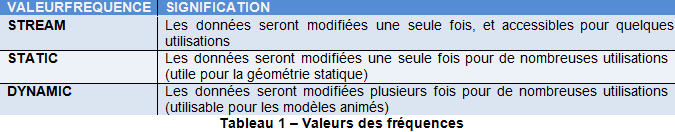
\includegraphics[width=15cm,height=2.94cm]{img/tableau1.png}
\\
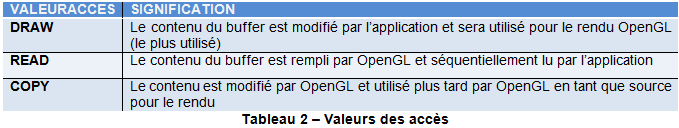
\includegraphics[width=15cm,height=3cm]{img/tableau2.png}

\subsubsection{Application d'un VA}
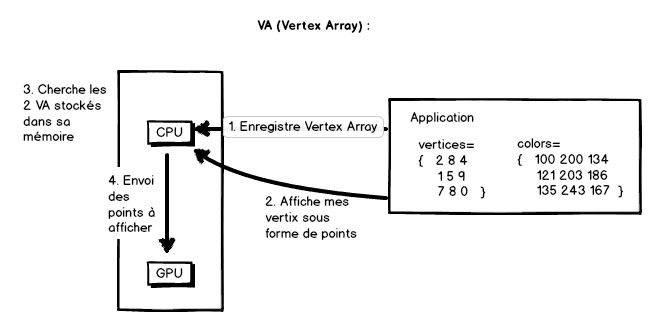
\includegraphics[width=15cm,height=7.48cm]{img/VA.png}
\subsubsection{Application d'un VBO}
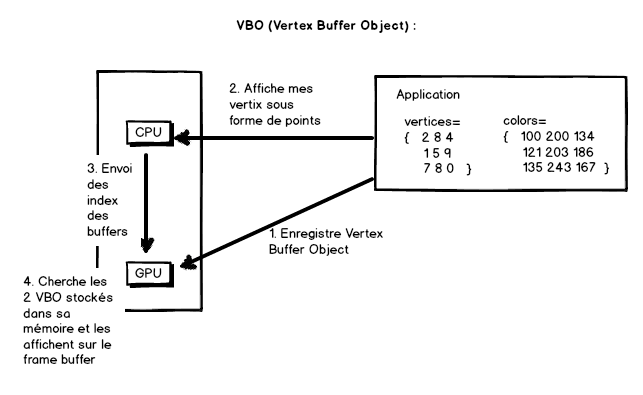
\includegraphics[width=15cm,height=9.26cm]{img/VBO.png}
\subsubsection{Application d'un VBO dans un VAO}
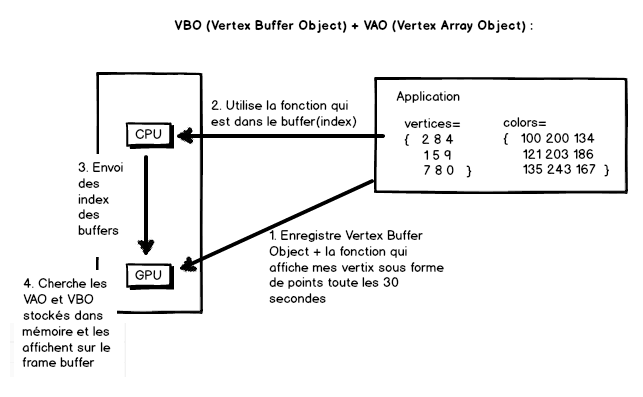
\includegraphics[width=15cm,height=9.21cm]{img/VAO_VBO.png}
%♥♥♥♥	♥♥♥♥